\documentclass[notes,11pt, aspectratio=169]{beamer}

\usepackage{pgfpages}
% These slides also contain speaker notes. You can print just the slides,
% just the notes, or both, depending on the setting below. Comment out the want
% you want.
\setbeameroption{hide notes} % Only slide
%\setbeameroption{show only notes} % Only notes
%\setbeameroption{show notes on second screen=right} % Both
\setbeamertemplate{caption}[numbered]
\usepackage{helvet}
\usepackage[default]{lato}
\usepackage{array}
\usepackage{natbib}
\usepackage{epstopdf}
\bibliographystyle{apalike}
\usepackage[affil-it]{authblk}
\usepackage{tikz}
\usepackage{verbatim}
\setbeamertemplate{note page}{\pagecolor{yellow!5}\insertnote}
\usepackage{amsmath}
\usepackage{mathpazo}
\usepackage{hyperref}
\usepackage{lipsum}
\usepackage{multimedia}
\usepackage{graphicx}
\usepackage{multirow}
\usepackage{graphicx}
\usepackage{dcolumn}
\usepackage{bbm}
\newcolumntype{d}[0]{D{.}{.}{5}}

\usepackage{changepage}
\usepackage{appendixnumberbeamer}
\newcommand{\beginbackup}{
   \newcounter{framenumbervorappendix}
   \setcounter{framenumbervorappendix}{\value{framenumber}}
   \setbeamertemplate{footline}
   {
     \leavevmode%
     \hline
     box{%
       \begin{beamercolorbox}[wd=\paperwidth,ht=2.25ex,dp=1ex,right]{footlinecolor}%
%         \insertframenumber  \hspace*{2ex} 
       \end{beamercolorbox}}%
     \vskip0pt%
   }
 }
\newcommand{\backupend}{
   \addtocounter{framenumbervorappendix}{-\value{framenumber}}
   \addtocounter{framenumber}{\value{framenumbervorappendix}} 
}


\usepackage{graphicx}
\usepackage[space]{grffile}
\usepackage{booktabs}

% These are my colors -- there are many like them, but these ones are mine.
\definecolor{blue}{RGB}{0,114,178}
\definecolor{red}{RGB}{213,94,0}
\definecolor{yellow}{RGB}{240,228,66}
\definecolor{green}{RGB}{0,158,115}
\definecolor{cardinalred}{RGB}{157,34,53}
\definecolor{appleblossom}{RGB}{255,255,255}
\definecolor{quartz}{RGB}{242,242,244}
\definecolor{graysquirrel}{RGB}{199,200,202}
\definecolor{spoofersstone}{RGB}{66,66,66}
\definecolor{blackwhetstone}{RGB}{0,0,0}


\hypersetup{
  colorlinks=false,
  linkbordercolor = {white},
  linkcolor = {blue}
}


%% I use a beige off white for my background
\definecolor{MyBackground}{RGB}{255,255,255}

%% Uncomment this if you want to change the background color to something else
%\setbeamercolor{background canvas}{bg=MyBackground}

%% Change the bg color to adjust your transition slide background color!
\newenvironment{transitionframe}{
  \setbeamercolor{background canvas}{bg=yellow}
  \begin{frame}}{
    \end{frame}
}

\setbeamercolor{frametitle}{fg=spoofersstone, bg=appleblossom}
\setbeamercolor{title}{fg=black}
\setbeamertemplate{footline}[frame number]
\setbeamertemplate{navigation symbols}{} 
\setbeamertemplate{itemize items}{-}
\setbeamercolor{itemize item}{fg=blue}
\setbeamercolor{itemize subitem}{fg=blue}
\setbeamercolor{enumerate item}{fg=blue}
\setbeamercolor{enumerate subitem}{fg=blue}
\setbeamercolor{button}{bg=MyBackground,fg=blue,}


% If you like road maps, rather than having clutter at the top, have a roadmap show up at the end of each section 
% (and after your introduction)
% Uncomment this is if you want the roadmap!
% \AtBeginSection[]
% {
%    \begin{frame}
%        \frametitle{Roadmap of Talk}
%        \tableofcontents[currentsection]
%    \end{frame}
% }
\setbeamercolor{section in toc}{fg=blue}
\setbeamercolor{subsection in toc}{fg=red}
\setbeamersize{text margin left=1em,text margin right=1em} 

\newenvironment{wideitemize}{\itemize\addtolength{\itemsep}{10pt}}{\enditemize}

\usepackage{environ}
\NewEnviron{videoframe}[1]{
  \begin{frame}
    \vspace{-8pt}
    \begin{columns}[onlytextwidth, T] % align columns
      \begin{column}{.58\textwidth}
        \begin{minipage}[t][\textheight][t]
          {\dimexpr\textwidth}
          \vspace{8pt}
          \hspace{4pt} {\Large \sc \textcolor{blue}{#1}}
          \vspace{8pt}
          
          \BODY
        \end{minipage}
      \end{column}%
      \hfill%
      \begin{column}{.42\textwidth}
        \colorbox{green!20}{\begin{minipage}[t][1.2\textheight][t]
            {\dimexpr\textwidth}
            Face goes here
          \end{minipage}}
      \end{column}%
    \end{columns}
  \end{frame}
}




\date{\today}
\title[]{\textcolor{cardinalred}{Challenges of Incorporating Rotation Information into Crop Insurance Rates}}
\author[VEF]{}
\institute[UARK]{\small{\begin{tabular}{c c c}
			Lawson Connor && Victor Funes-Leal && Eunchun Park\\
			\multicolumn{3}{c}{\small Department of Agricultural Economics and Agribusiness}\\ 
			\multicolumn{3}{c}{\small University of Arkansas}\\
\end{tabular}}}
 
\makeatletter

\begin{document}

% logo of my university  
%\logo{\includegraphics[width=2.5cm]{figures/ACES-Logo.pdf}}
\titlegraphic { 
\begin{tikzpicture}[overlay,remember picture]
\node[right = 0.2cm] at (current page.200){
    
\includegraphics[width=3cm]{figures/UA_Logo.eps}
};
\end{tikzpicture}
}
	
	%%% TIKZ STUFF
	\tikzset{   
		every picture/.style={remember picture,baseline},
		every node/.style={anchor=base,align=center,outer sep=1.5pt},
		every path/.style={thick},
	}
	\newcommand\marktopleft[1]{%
		\tikz[overlay,remember picture] 
		\node (marker-#1-a) at (-.3em,.3em) {};%
	}
	\newcommand\markbottomright[2]{%
		\tikz[overlay,remember picture] 
		\node (marker-#1-b) at (0em,0em) {};%
	}
	\tikzstyle{every picture}+=[remember picture] 
	\tikzstyle{mybox} =[draw=black, very thick, rectangle, inner sep=10pt, inner ysep=20pt]
	\tikzstyle{fancytitle} =[draw=black,fill=red, text=white]
	%%%% END TIKZ STUFF

 
	% Title Slide
 
\begin{frame}
	\maketitle
	\centering 
\end{frame}

\begin{frame}{Outline}
\begin{wideitemize}
    \item \emph{Research Question}: How do long-term crop rotation patterns affect corn yields?
    \item \emph{Method}: We use linear fixed effects models to quantify the magnitude of the relationship between yields and rotational complexity.
    \item \emph{Data}: Yield (biomass) data from \cite{lobell2015} (SCYM) and \cite{Ma2024} (QDANN), Rotational complexity index, from \cite{socolar2021}, field-level crops (CDL), and weather variables (PRISM).
    \item \emph{Results}: The effect of rotations on yields depends critically on their timing; later soybean rotations and shorter gaps between soy harvests have more positive and significant effects on yields.
    \item However, more and less spaced-out soy harvests have negative and significant effects on corn yields.
\end{wideitemize}
\end{frame}

\begin{frame}{Background}
    \begin{wideitemize}
        \item Interest in incorporating farm-level conservation practices into crop insurance rates?
        \begin{itemize}
            \item Cover cropping
            \item No till farming
            \item Crop rotations (corn and soybeans plus other crops)
        \end{itemize}
        \item These practices are thought to reduce yield risk, but may adversely affect short-term yields and farmer premium rates through their APH.
        \item Potentially reduce practice adoption incentives
    \end{wideitemize}
\end{frame}

\begin{frame}{Crop Rotation and Farm Production}
\begin{wideitemize}
    \item Increased rotation shown to have agroecological benefits for farm production, particularly in the face of adverse weather events \citep{socolar2021, burchfield2024}.
    \item Rotations help maintain soil organic carbon and fertility and reduce yield variability \citep{wu2025}. Still, this effect is conditional on soil characteristics (higher yield boost in lower productivity areas).
    \item Corn and soy rotations are the most prevalent in the US Midwest
    \item Challenges exist from a rating perspective for incorporating crop rotations into the rates.
\end{wideitemize}
\end{frame}

\begin{frame}{Measuring Rotation Patterns}
\begin{wideitemize}
    \item There are several ways to measure ecological diversity
    \begin{enumerate}
        \item Rotational Complexity Index (RCI)
        \item Landscape Diversity Index
        \item Entropy-based measures
        \item Diversity indexes (weighted average of each number of crops)
    \end{enumerate}
    \item Values of these indices can be incorporated into the rating system
    \item However, yields and yield risk are not a linear function of diversity indices, which presents a challenge for rating.
\end{wideitemize}
\end{frame}

\begin{frame}{Objectives}
\begin{wideitemize}
    \item Show that RCI has a nonlinear effect on yield and yield risk.
    \item Determine identifiable indicators in a 6-year corn soy. rotation that affect yield and yield risk.
    \item Develop a rotation score and rank 6-year rotations using score.
\end{wideitemize}
\end{frame}


\begin{frame}{Data}
    \begin{wideitemize}
        \item \textbf{Scalable Satellite-Based Crop Yield Mapper (SCYM) yield data}: \citep{lobell2015} relies on a large number of crop model simulations over a range of soil, climate, and management conditions daily to train a statistical model at a pixel level, which is used to predict field-level biomass that can be converted to yields.
        \item \textbf{Quantile loss Domain Adversarial Neural Networks (QDANN) yield data}: \citep{Ma2024} uses county-level yields and field-level data to train a neural network, which is, in turn, used to predict yields at the field level using a technique called \textit{Unsupervised domain adaptation} (UDA).
        \item Both models use Landsat data as their main input, along with Gridmet data to calibrate yield models at a 30m resolution.
        \item Reported accuracy for QDANN is higher than that of SCYM (35\% for SCYM versus 48\% for QDANN at a field level).
    \end{wideitemize}
\end{frame}

\begin{frame}{Methods: First Moment of Yield}
\begin{wideitemize}
    \item We model the conditional moments from the yield distribution as:
        \begin{equation*}
    yields_{it}=seq_{it}+W_{it}\beta_{it}+\lambda_{k}+\gamma_{t}+\varepsilon_{it}
        \end{equation*}
    \item $yields_{it}$: corn yields (in bushels per acre) of field $i$ in year$t$.   
    \item $seq_{it}$: is a categorical variable for each rotation sequence, with corn monoculture as the base category.
    \item $W_{it}$: controls (precipitation, mean temperatures, VPD, PDSI, NCCPI, soil characteristics).
    \item $\lambda_{k}$, $\gamma_{t}$ are FIPS and year fixed effects.
\end{wideitemize}
\end{frame}

\begin{frame}{Methods: Second Moment of Yield}
   \begin{wideitemize}
    \item Let $\hat{u}_{1}$ be the associated error term, such that: $\hat{u}_{1}=y-X\hat{\beta}_{1}$, $X=\left[Z, W \right]$, then all higher moments can be estimated as:
    \begin{equation*}
        (\hat{u}_{1})^{i} = M_{i}(X,\beta_{i})+\varepsilon_{1}=X\beta_{i}+\varepsilon_{1}
    \end{equation*}
    \item Coefficients $\hat{\beta}_{1}$ can be consistently estimated using OLS with heteroskedasticity-consistent standard errors \citep{shi2013} or using bootstrap \citep{li2021}.
    \item We can quantify the differential impacts of every rotation sequence on the risk by examining the coefficients in the regression of $X$ on $\hat{u}_{1}^{2}$ \citep{antle1983}.
    \end{wideitemize}
\end{frame}

\begin{frame}{Relationship between RCI and Yields in a two-crop rotation}
    \begin{figure}[H]
    \centering
    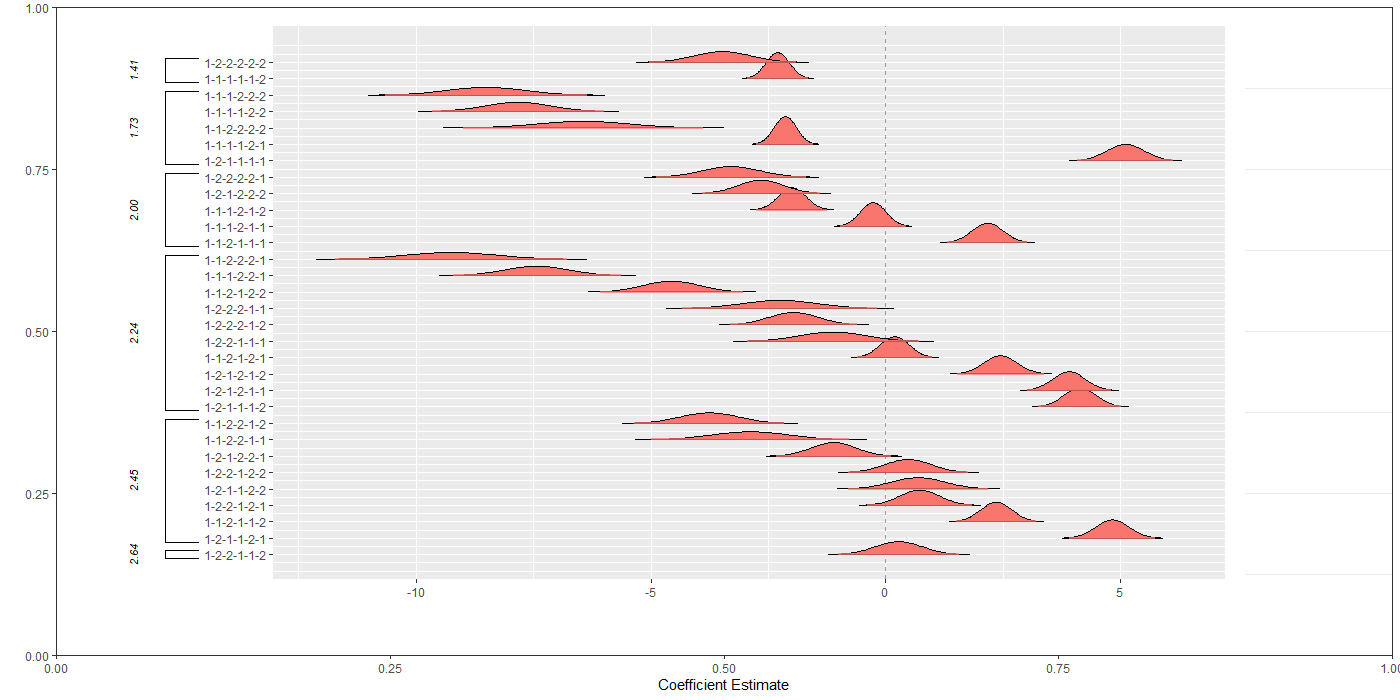
\includegraphics[scale = 0.35]{figures/rci_coeff.png}
    \caption{Response of yields to rotation sequences}
    \label{fig:crop_rotation_yields} 
    \end{figure}
\end{frame}

\begin{frame}{General Findings}

    \begin{wideitemize}
        \item Only a few sequences outperform corn monoculture in terms of higher mean/lower variance.
        \item Both SCYM and QDANN yield similar results. 
        \item Higher performing sequences have common elements:
        \begin{enumerate}
            \item A recent soy rotation (year 1 or 2).
            \item No consecutive soy years.
            \item Low impact of older crops (first three years).
            \item Perfect corn/soy rotation has positive but nonsignificant effects on yields, and reduces yield variance.
        \end{enumerate}
    \end{wideitemize}
\end{frame}

\begin{frame}{Key Indicators Idntified}
    \begin{wideitemize}
        \item We identified a set of rotation patterns that account for variations in first and second moments of corn yields.
        \begin{enumerate}
            \item Soy Lag: equal to the number of lagged periods a soy harvest was detected since the most recent year (e.g. if the latest soy harvest was the previous year, it takes a value equal to -1).
            \item Consecutive soy years: Dummy equal to 1 if a rotation pattern had two or more consecutive soy harvests.
            \item Soy gap: minimum number of years between two soy harvests (e.g. if two years of soy harvests occur, then the soy gap is 0).
            \item Number of soy harvests: how many times in the last seven years was a soy harvest detected?
        \end{enumerate}
    \end{wideitemize}
\end{frame}

\begin{frame}{Rotation sequences and yields (QDANN)}
    \begin{figure}[H]
    \centering
    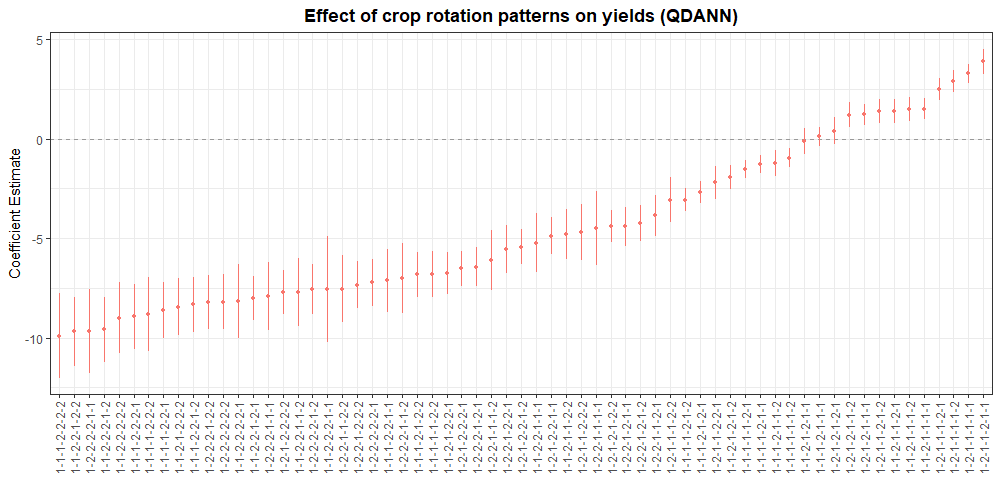
\includegraphics[scale = 0.5]{figures/qdann_means.png}
    \caption{Coefficients of rotation sequences}
    \label{fig:qdann_means} 
    \end{figure}
\end{frame}

\begin{frame}{Rotation sequences and yields}
    \begin{wideitemize}
    \item We model average yields as a linear FE model:
        \begin{equation*}
            y_{it}=Z\tau_{it}+W_{it}\beta_{it}+\lambda_{k}+\gamma_{t}+\varepsilon_{it}
        \end{equation*}
        \item Where: $Z = \left[late\_soy, soy\_cons,soy\_gap, nsoy\right]$
    \end{wideitemize}
\end{frame}

% calculate the score for each rotation type
% latest soy rotation
% soy gap
% number of soy harvests
% add a slide of coefficients ordered by score

\begin{frame}{Coefficient estimates}
    
\begin{table}[htbp]
   \caption{\label{tab:fit1} Effect of rotation patterns on yields}
   \bigskip
   \centering
   \resizebox{0.85\textwidth}{!}{
   \begin{tabular}{lcccc}
      \toprule
      Variable                        & QDANN mean      & SCYM mean           & QDANN variance & SCYM variance \\   
      \midrule 
      Latest soy rotation             & 2.847$^{***}$   & 3.550$^{***}$       & -9.017$^{**}$  & 5.826\\   
                                      & (0.1663)        & (0.2167)            & (4.318)        & (6.843)\\   
      Soy gap                         & 0.3114$^{***}$  & 0.2466$^{***}$      & 2.611$^{**}$   & 6.177$^{***}$\\   
                                      & (0.0407)        & (0.0499)            & (1.181)        & (1.646)\\   
      Number of soy harvests          & -0.9760$^{***}$ & -1.080$^{***}$      & -11.17$^{***}$ & -32.93$^{***}$\\   
                                      & (0.1341)        & (0.1587)            & (3.198)        & (4.268)\\   
      Number of consecutive soy years & -4.671$^{***}$  & -4.171$^{***}$      & 79.18$^{***}$  & 133.9$^{***}$\\   
                                      & (0.2270)        & (0.2566)            & (5.649)        & (7.589)\\   
      Controls                        & Yes             & Yes                 & Yes            & Yes\\  
       \\
      Observations                    & 1,744,038       & 1,411,846           & 1,744,038      & 1,411,846\\  
      R$^2$                           & 0.57998         & 0.62967             & 0.05231        & 0.03429\\  
      Within R$^2$                    & 0.20564         & 0.17989             & 0.01483        & 0.00676\\  
       \\
      year fixed effects              & $\checkmark$    & $\checkmark$        & $\checkmark$   & $\checkmark$\\   
      fips fixed effects      & $\checkmark$    & $\checkmark$        & $\checkmark$   & $\checkmark$\\   
      \bottomrule
   \end{tabular}}
\end{table}



\end{frame}

\begin{frame}{Rotation Score Generation}
\begin{wideitemize}
    \item All four variables can be used to construct a \textbf{rotation score}:
    \begin{equation*}
        score_{it}=\hat{\beta}_{1}late\_soy_{it}+\hat{\beta}_{2}soy\_cons_{it}+\hat{\beta}_{3}soy\_gap_{it}+\hat{\beta}_{4}nsoy_{it}
    \end{equation*}
    \item This score summarizes the information from the four variables and allows us to classify the 64 rotation patterns into a smaller set of values.
    \item Score values for corn monoculture are 0, and for perfect rotation, 2.59.
    \item We predict yields based on rotation score and summarize our findings.
    \end{wideitemize}
\end{frame}

\begin{frame}{Relationship between score and Yields in a two-crop rotation}
    \begin{figure}[H]
    \centering
    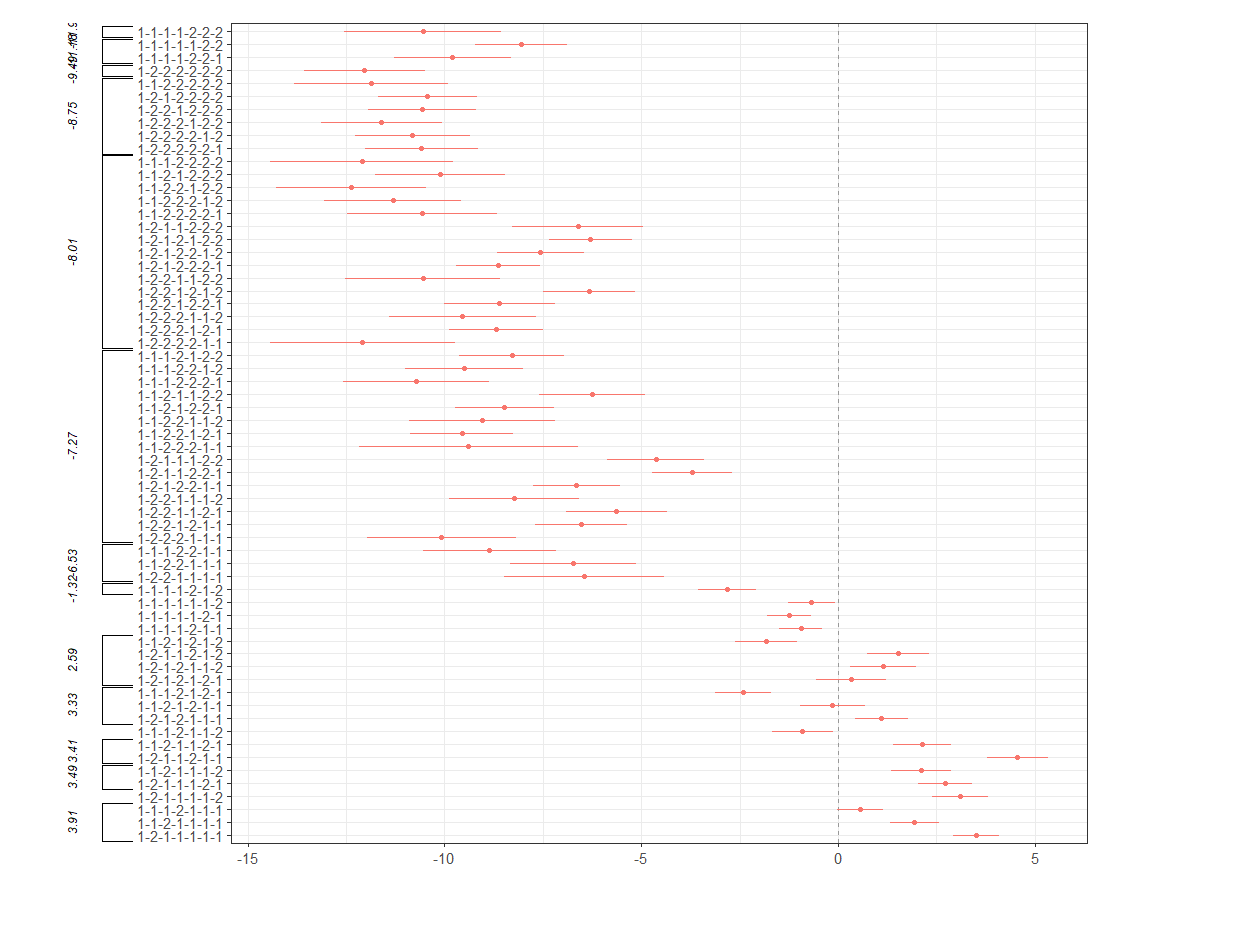
\includegraphics[scale = 0.4]{figures/rot_score.png}
    \caption{Response of yields to rotation sequences}
    \label{fig:rot_score} 
    \end{figure}
\end{frame}

\begin{frame}{Relationship between score and Yields in a two-crop rotation}
    \begin{figure}[H]
    \centering
    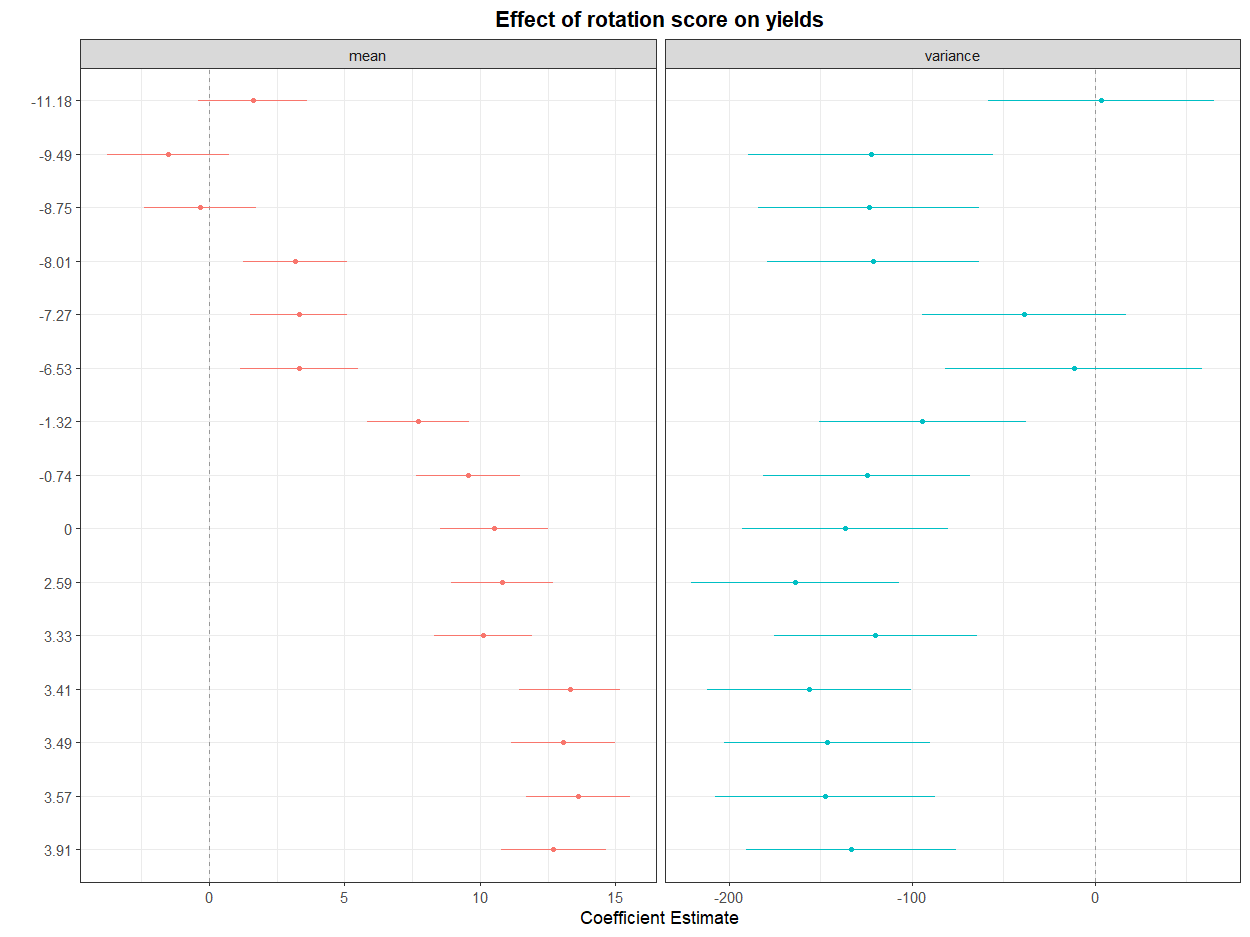
\includegraphics[scale = 0.35]{figures/mean_var_score.png}
    \caption{Response of yields to score values}
    \label{fig:rot_score} 
    \end{figure}
\end{frame}

\begin{frame}{Next Steps}
    \begin{wideitemize}
        \item Having a rotation score that predicts yields allows us to perform causal identification of the effect of shifting rotations on yield outcomes. 
        \item What are the main factors driving rotation choices?
        \begin{itemize}
        \item Changes in Output prices (corn vs soybeans).
        \item Changes in input prices \citep{gammans2025}.
        \item Weather variations \citep{pates2021}.
        \item Distance to ethanol plants \citep{cheu2025, pates2025}.
        \end{itemize}
        \item Can incorporate scores into a rating formula
    \end{wideitemize}
\end{frame}

\begin{frame}{Determinants of crop choices}
    \begin{figure}[H]
    \centering
    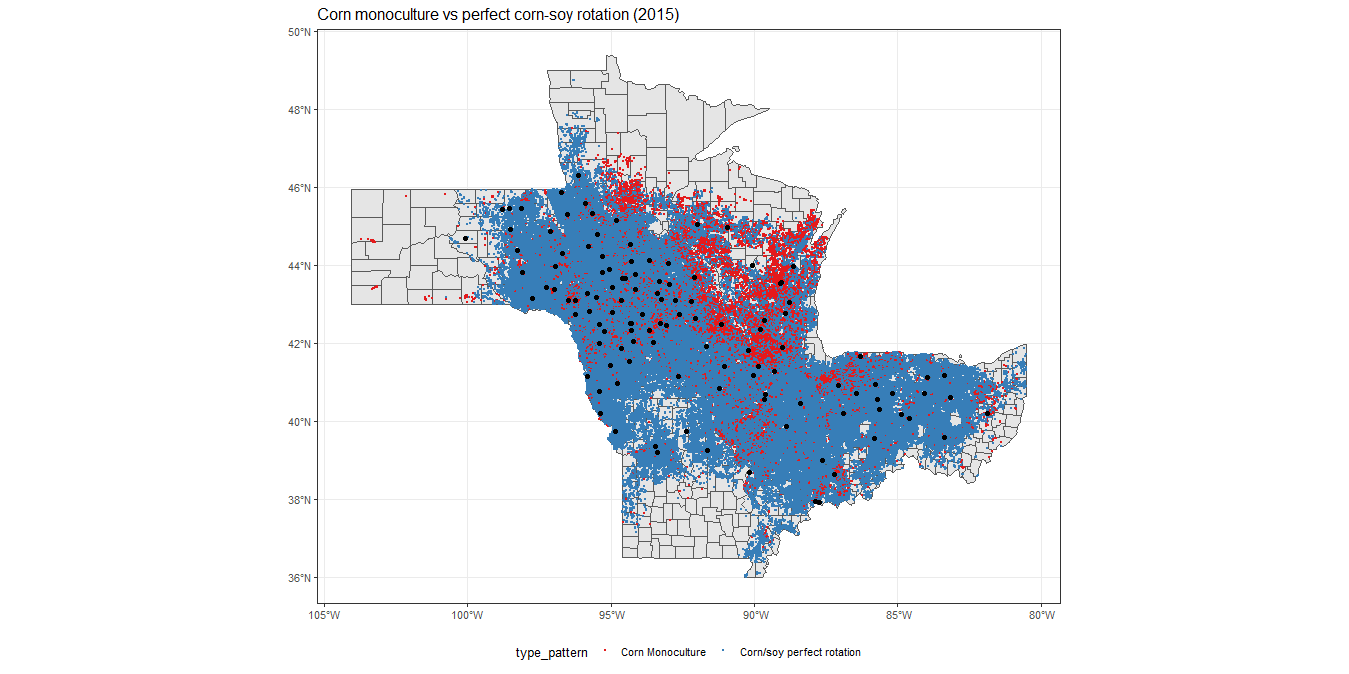
\includegraphics[scale = 0.35]{figures/corn_map.png}
    \caption{Corn monoculture vs. perfect rotation and location of ethanol plants}
    \label{fig:corn_map} 
    \end{figure}
\end{frame}

\begin{frame}{}
	\centering \Huge
	\emph{Thank You!}
\end{frame}
	
\begin{frame}[allowframebreaks]{References}
	\bibliography{bibliography.bib}	
\end{frame}	
\end{document}